\section{Theoretical Model}
\label{sec:section2}
\subsection{Setup}\label{sec:section2.1} 
Throughout this section, I establish the theoretical framework for the model considered in this paper. Fix a non-atomic continuum of male and female agents and consider the dynamic two-sided market formed by the SBDA platform, which agents can join to search for potential romantic partners. 
For ease of exposition, I assume that this market is heteronormative such that male agents search exclusively for female agents and vice-versa. 
Time is discrete and indexed $t=0, 1, 2, ...$ over an infinite horizon. 
At every time period, agents from each sex are paired and presented a candidate partner from the opposite side of the market.  
\begin{comment}
    Each agent has an attractiveness type $\theta \in \Theta := [0,1]$ which is unknown to them but observable to their candidate, and it is common knowledge that this is the case.
\end{comment}
We model agents with heterogeneous preferences (capturing the notion that `beauty lies in the eye of the beholder') and thus, after being paired, each agent observes an \textit{idiosyncratic attractiveness value} $\theta \in \Theta := [0,1]$ for their candidate. These values are drawn i.i.d from distributions with CDF's $F_m, F_w$, with female agents drawing male candidate values from $F_m$ and vice versa. Importantly, the value men $i$ draws for women $j$ does not necessarily equal the value that $j$ draws for $i$, and, for simplicity, these are modelled these as independent from one another.

After observing their candidate's attractiveness, agents then choose whether to swipe left (dislike) or right (like) on them, yielding an action space of $\mathcal{A}=\{ \text{left},\; \text{right}\}$. 
If both agents swipe right on one another, they are said to have \textit{matched} and both receive a matching payoff, however, if either agent swipes left, they both receive a payoff of zero. Contingent on swiping right on a candidate with attractiveness $\theta$, a user earns a matching payoff $u(\theta)$, where $u(\cdot)$ is a continuous, strictly increasing function that satisfies $u(0) = 0$. 
This last property stems from the fact that, in Tinder, users are allowed to unmatch with each other, thus implying that matching with the least attractive individual on the other side of the market is weakly preferred to not matching. 

After payoffs have been received, players are paired to different candidates and the stage interaction is repeated. Given the continuum of agents, I assume that interactions take place \textit{anonymously} in the style of \cite{jovanovic1988anonymous}. Furthermore, to the agents' knowledge, pairings are determined in an unknown manner (since SBDA's are generally secretive regarding the algorithms used), effectively making their problem one of uniform random search.

\begin{figure}[ht]
    \centering 
    \caption{Sequence of events within each time period}
    \vspace{20pt} 
        \begin{tikzpicture}
            % draw horizontal line   
        \draw[thick, -Triangle] (0,0) -- (\ImageWidth,0); %node[font=\scriptsize,below left=3pt and -8pt]{$t+1$};

        % draw vertical lines
        \foreach \x in {1,2,...,6}
        \draw (\x*2 cm,4pt) -- (\x*2 cm,-4pt);

        \foreach \x/\descr in {2/t, 4/\text{Arrivals}, 6/\text{Pairings}, 8/\text{Game Play}, 10/\text{Departures}, 12/t+1}
        \node[font=\scriptsize, text height=1.75ex,
        text depth=.5ex] at (\x,-.3) {$\descr$};  
    \end{tikzpicture}
    \label{fig:timeline}
\end{figure}

Perhaps trivially, swiping right in the stage interaction described above is both weakly dominant for all agents and yields a Pareto-optimal outcome, thus implying that, in a repeated interaction, the market equilibrium would have all agents exclusively swiping right. Despite this, the main selling point of SBDA's is a reduction in searching costs for individuals seeking romantic encounters, and this is only accomplished if matches have a high likelihood of resulting in real-life romantic attraction. Because of this, SBDA's like Tinder place a cap on the total number of right swipes for each user, thus enabling this as a form of costly signalling. I refer to the total number of right-swipes a user has left as its \textit{budget}, $b_t$, which evolves dynamically according to the law of motion:

\begin{equation*} 
  b_{t+1}= b_{t}- a_{t} 
\end{equation*}

where the budget caps for each sex, $B_m$ and $B_w$, are determined exogenously. The budget sets for men and women are thus defined by $\mathcal{B}_{s}=\{b \in \mathbb{Z} : 1\leq b \leq B_s\}$, for each sex $s=m,w$. Each period, new men and women enter the platform at rates $\lambda_m, \lambda_w>0$.
\begin{comment}
    , with their attractiveness drawn i.i.d from distributions with cumulative distribution functions $F_m$ and $F_w$, respectively
\end{comment}
Importantly, agents depart from the platform in one of two ways: they can leave \textit{endogenously}, if they expend their swiping budget, or \textit{exogenously} with probability $(1-\delta)$. This admits to the interpretation of a geometrically distributed lifetime within the platform, parametrised by $\delta$, and implies that users use this as a discounting factor for future payments.

Due to the anonymity assumption above, agents can relax history-related considerations, essentially simplifying their stage problem to one that depends on the candidate attractiveness and their own budget only. Due to this, I restrict focus to stationary Markovian strategies, denoted by $\mu: \Theta \times\mathcal{B}_m\rightarrow \Delta\mathcal{A}_m$ for men and $\omega:\Theta \times\mathcal{B}_w\rightarrow \Delta\mathcal{A}_w$ for women, where $\Delta S$ denotes the probability simplex over set S. 

\subsection{The Dating Market}\label{sec:section2.2}
Given the sequence of events taking place in the stage interaction, I now outline the system state variables that make up the Tinder market. Let $N_{mt}(b), N_{wt}(b)$ denote the mass of male and female agents (respectively) with a budget of $b\in\mathcal{B}$ in a given time period $t$. Furthermore, since gender imbalances can leave some agents in the long side of the market unpaired, a pairings process must be fixed. Given fairness considerations as well the automated nature of SBDA platforms, I assume an efficient matching technology and model pairings as a Bernoulli process parametrised by market tightness; thus, the probability of being paired with a candidate is defined for both sides as:

%These are endogenously determined since the flow of agents into lower budget levels and eventually out of the platform depends on their swiping decisions.

\begin{equation*}
    \tau_{mt}:=\min \Big\{\frac{N_{wt}}{N_{mt}} ,1 \Big\}, \quad \tau_{wt}:= \left(\frac{N_{mt}}{N_{wt}}\right) \tau_{mt} 
\end{equation*}


From the above, the platform state at time period $t$ can be defined as $\Psi_t=(N_{mt},N_{wt})$. For most of this paper, I focus on characterising user behaviour and its resulting implications in a stationary setting (which is denoted by omitted time subscripts), although some discussion of coupled strategy and market dynamics is provided in \autoref{sec:section4}. As a necessary requirement, the market steady state $\Psi_t=\Psi_{t+1}=...=\Psi$ must satisfy the balanced flow conditions \footnote{Formally, these conditions rely on the exact law of large numbers, which has been rigorously developed for discrete-time settings by \cite{duffie2018dynamic}, but a technical discussion of this lies outside the scope of this paper} for our continuum model; these are presented below for the female agents, but they apply analogously to the male side of the market. Firstly, the entry flow of agents into the platform must equal the departure flow: 

% Budget dist equations
\begin{equation}\label{eq:ss1} 
    \lambda_w\;=\; \underbrace{ (1-\delta)\sum_{b\in\mathcal{B}_w}N_w(b)}_{\text{Exogenous Outflow}} \;+\; \underbrace{N_w(1) \delta \tau_w\int_{\Theta}\omega(\theta,1)\,dF_{m}(\theta)}_{\text{Endogenous Outflow}} 
\end{equation} 

Secondly, for both sides, the flow of agents into any particular budget level must equal the outflow of agents from that same level. Thus, for all $b\in\mathcal{B}_w$: 

\begin{equation}\label{eq:ss2} 
    \underbrace{N_w(b+1) \delta \tau_w \int_{\Theta} \omega(\theta,b+1)\,dF_{m}(\theta)}_{\text{Inflow into $b$}} \;=\; \underbrace{N_w(b) \Big[ (1-\delta) \;+\; \delta \tau_w\int_{\Theta} \omega(\theta,b)\,dF_{m}(\theta)\Big]}_{\text{Outflow from $b$}}
\end{equation}

Finally, the entry flow of agents into the platform must equal the outflow from the top budget level, hence:

\begin{equation}\label{eq:ss3} 
    \lambda_w \;=\; \underbrace{N_w(B_w) \Big[ (1-\delta) \;+\; \tau_w \delta \int_{\Theta} \omega(\theta,B_w)\,dF_{m}(\theta) \Big]}_{\text{Outflow from $B_w$}}
\end{equation} 

\subsection{The Search Problem}\label{sec:section2.3}
With the model framework and market dynamics outlined above, I now explore the decision problem faced by female agents in the market, with analogous results and implications for the male side. In the discussion below, I derive the female best-response function given a fixed, stationary market state $\Psi$ and male strategy $\mu$. To begin this analysis, consider a woman $i$ who is paired with a man $j$ in Tinder. The expected ex-interim payoff for this women, given that she observes attractiveness $\theta$ for candidate $j$ and chooses action $a$, is the following:

\begin{equation*}
    \begin{aligned}
        U(\theta, a)&=\Big(\overline{\mu}\,\mathbbm{1}\{a=\text{right}\}\Big)\,u(\theta), \quad \text{where}\quad \overline{\mu} &= \sum_{b\in \mathcal{B}_m}\int_{\Theta} \mu(\theta',b)\,{N}_m(b)\,dF_w(\theta')
    \end{aligned} 
\end{equation*}

Here, $\overline\mu$ denotes candidate $j$'s strategy averaged over the possible attractiveness values that he may observe for $i$ and his possible budget level, both of which are unknown to woman $i$. The payoff function above imposes a mean-field assumption where, conditional on the fixed platform state $Psi$, woman $i$ averages out her opponent's strategy, rather than considering candidate $j$'s specific behaviour and beliefs over his possible budget level. This modelling choice has been employed by \cite{immorlica2021designing} and \cite{iyer2014mean} among others, as it simplifies the full-fledged dynamic game by collapsing it onto a pair of Markov Decision Processes (MDP's), where strategy $\omega$ is a best response for female agents if and only if it is an optimal policy for the corresponding MDP. Consider the arrival times of the realized pairing process for woman $i$ and index these by $k$. Given that, at the time of pairing, this women has a budget of $b$ right swipes left, she then solves the constrained MDP presented below, captured by the value function $V_w(\theta,b)$:

\begin{equation*}
    \begin{aligned} 
        V_w(\theta,b)=\max_{\{a_t\}^\infty_{t=0}} \quad & \mathbb{E}_{\theta}\left[\sum^\infty_{t=0} \delta^{t} U(\theta_t, a_t) \;|\; \theta_0=\theta, b_0=b\right]\\ 
        \textrm{s.t.} \quad & b_{t+1} = b_t -a_t \\
        & b_t\in \mathcal{B}_w \cup \{0\} \\
        & a_t\in \mathcal{A}  
    \end{aligned}
\end{equation*}

Importantly, the first two constraints along with the exogenous departure process make this problem non-trivial; by limiting woman $i$'s right-swiping budget, the platform imposes an opportunity cost between swiping right on man $j$ and foregoing potential future matches with more attractive men, whilst the exogenous departure process removes the possibility of simply waiting around to swipe right on the top $B_w$ most attractive men. By standard dynamic programming arguments, this problem can be captured by two Bellman equations; one for when $j$ is paired and another for when she isn't:

\begin{align}
    \begin{split} 
        V^{P}_w(\theta,b) &=\max \Big\{ \, \overline{\mu}\, u(\theta) \;+\; \delta \tau_w \,\mathbb{E}_\theta \Big[V^P_w(\theta', b-1)\Big] \;+\; \delta (1-\tau)V^{NP}_w(b-1) \, ,\\[6pt]
        & \quad\quad\quad\quad\;\delta \tau_w \, \mathbb{E}_\theta\Big[ V^P_w(\theta', b) \Big] \;+\; \delta (1-\tau_w) V^{NP}_w(b) \, \Big\}
    \end{split}\\[10pt]
    \begin{split}
        V^{NP}_w(b) &= {}\delta \tau_w \,\mathbb{E}_\theta \Big[ V^P_w(\theta', b)\Big] \,+\, \delta (1-\tau_w) V^{NP}_w(b)
    \end{split} 
\end{align} 

With some straightforward algebra, the above two equations can be merged into the full Bellman equation below. Note that, to impose the swiping budget constraint from the above MDP, it must be the case that $V(\theta, 0)=0, \; \forall \theta \in \Theta$, since agents with no right-swipes left must leave the platform and can't accumulate any additional payoffs:

\begin{equation}
    \begin{aligned} 
        V_w(\theta,b) \;=\;&\max\left\{\,\overline{\mu} \, u(\theta) +\alpha \,\mathbb{E}_\theta \Big[V_w(\theta', b-1)\Big]\,,\; \alpha\,\mathbb{E}_\theta \Big[ V_w(\theta', b)\Big]\,\right\}
    \end{aligned}
\end{equation}

Where $\alpha$ is the effective discount rate accounting for the exogenous possibilities of both departures and pairings, defined as: 

\begin{equation*}
\alpha:=\frac{\tau_w\delta}{1-\delta(1-\tau_w)}
\end{equation*}

Upon inspection, it is clear that the value function is of a piecewise nature in $\theta$; thus, the optimal policy can be determined by a set of reservation attractiveness levels, $\{\tilde\omega\}_{b\in \mathcal{B}_w}$, where women $j$ swipes right for partners who exceed the reservation level for her current budget. These reservation levels must be such that woman $i$ is indifferent between swiping left or right, thus:

\begin{equation*}
    \begin{split}
        \omega(\theta,b)&=\begin{cases}
            1,\quad \theta\geq \widetilde{\omega}_b \\ 
            0, \quad\theta< \widetilde\omega _b  
        \end{cases} , \quad \text{where $\widetilde{\omega}_b$ satisfies:} \\[8pt] 
        \overline\mu u(\widetilde\omega_b) &= \alpha \, \mathbb{E}_\theta\Big[\,V(\theta',b)-V(\theta',b-1)\,\Big]  
    \end{split}
\end{equation*} 

Although reservation attractiveness levels can be computed using numerical algorithms such as value or policy iteration \citep{rust1987optimal}, they are more explicitly characterized by the result below (with a corresponding proof included in \autoref{appx: b}): 

\begin{proposition}
The set of reservation attractiveness levels for women, $\{\tilde\omega_b\}_{b\in \mathcal{B}_w}$, uniquely satisfies the recurrence relation and initial condition below, over the budget set $\mathcal{B}_w$: 

\begin{equation}\label{eq:recurrence relation}
    \begin{aligned}
        u(\widetilde \omega_b) \;=\; \alpha u(\widetilde \omega_b) F_m(\widetilde \omega_b) \;+\; \alpha u(\widetilde \omega_{b-1}) \Big[1- F_m(\widetilde \omega_{b-1})\Big] \;+\; \int^{\widetilde \omega_{b-1}}_{\widetilde \omega_b} \alpha u(\theta')\,dF_m(\theta')
    \end{aligned} 
\end{equation} 

\begin{equation}\label{eq:initial condition}
    u(\widetilde\omega_1) \;=\; \alpha u(\widetilde\omega_1)F(\widetilde\omega_1) \;+\; \alpha \int^1_{\widetilde\omega_1}u(\theta')dF(\theta')
\end{equation}
\end{proposition} 

%This result (with a corresponding proof included in \autoref{appx: b}), allows for improved computation of agent best-responses as it removes the need to discretise $\Theta$ (which is required when applying the above methods to uncountable state spaces), and it provides improved performance compared to the above methods, with a typical runtime complexity of $\mathcal{O}(|\mathcal{A}||\Theta \times \mathcal{B}_w|^2)$. 
\begin{figure}[ht]
    \centering
    \caption{The Optimal Swiping Rule}
    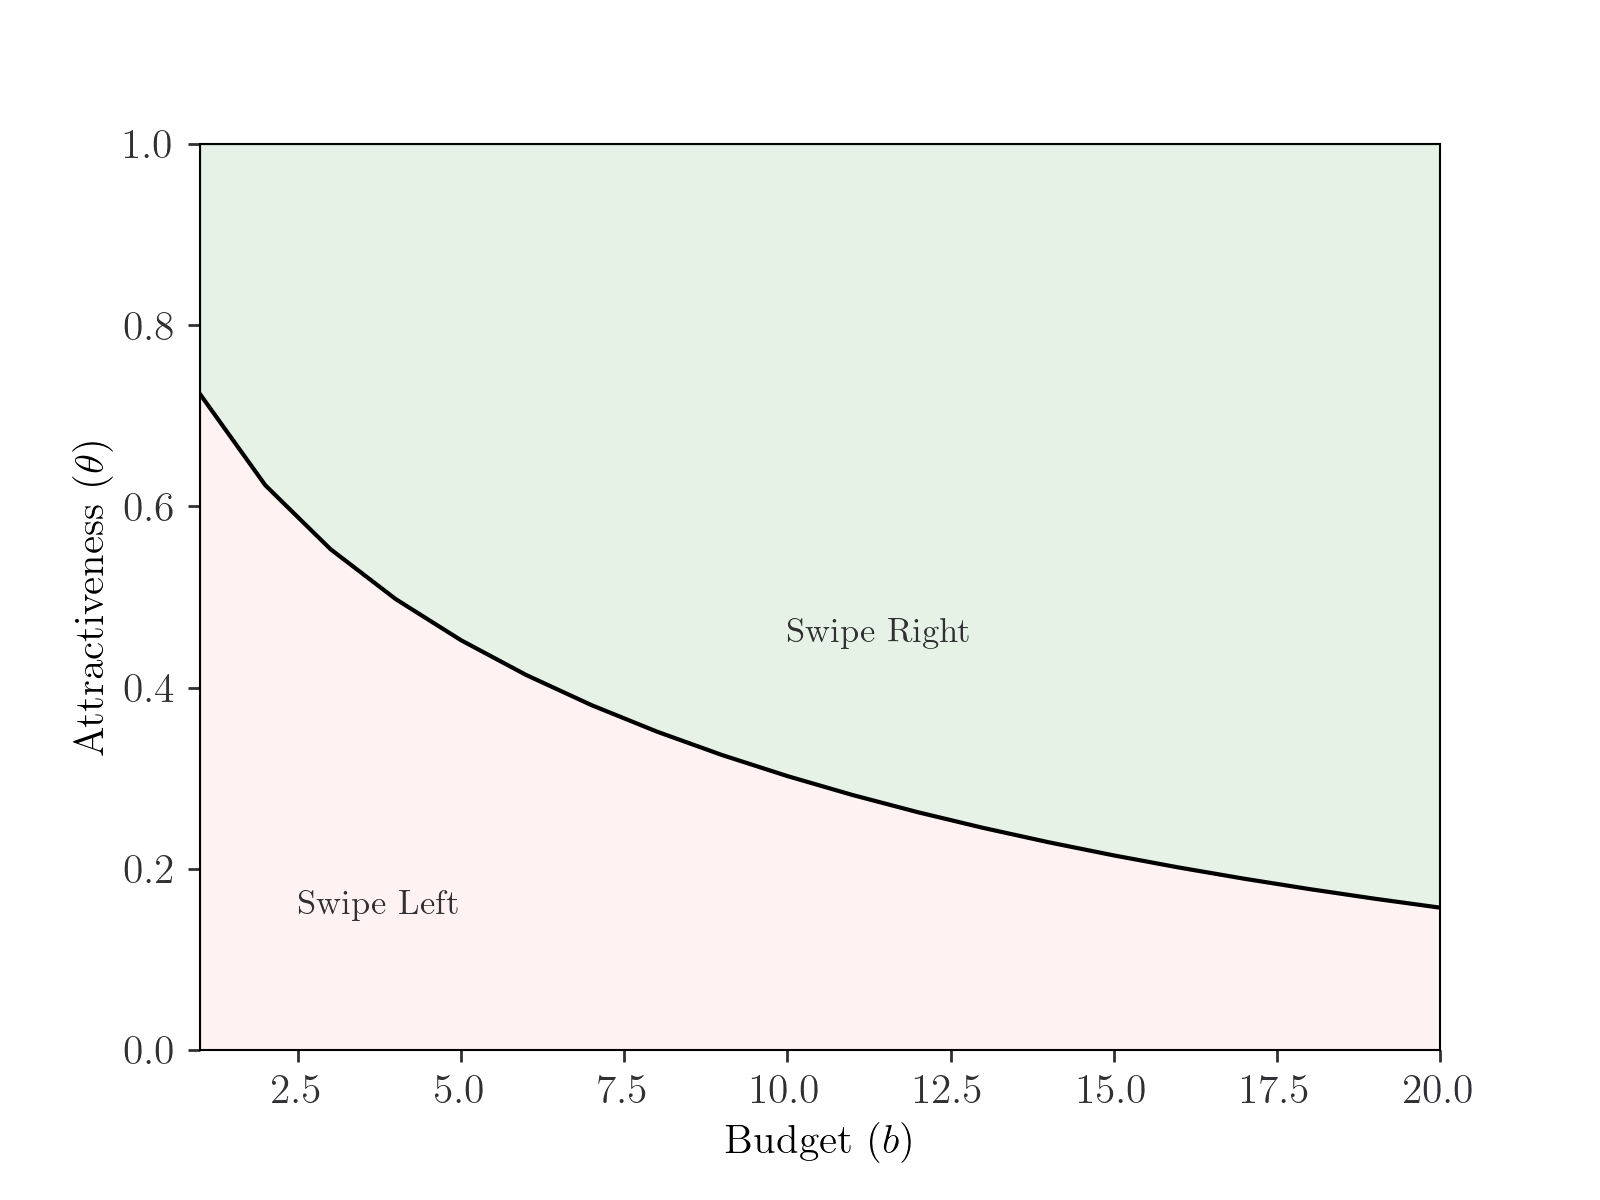
\includegraphics{swiping-rule.png}
    \label{fig:swiping-rule} 
\end{figure}

By further inspecting this result, it is evident that the aggregate behaviour of the opposite side of the market ($\overline\mu$) has no direct influence over female best responses. Instead, this influence happens indirectly through the steady state masses and their effect on how agents discount inter-temporal payoffs through $\alpha$. Using the recurrence relation in Proposition 1, the agent-best response was computed for an arbitrary set of exogenous parameters, with results shown in \autoref{fig:swiping-rule}. As evidenced by these, the optimal policy (and best-response function) for agents is marked by a clear cut-off rule for swiping right. These cut-off values are decreasing in the agent's budget, which captures the notion that an agent's current swipe is more valuable than all preceding ones given the increasing opportunity cost.  
